%=============================================================================
%   Pentomino by Pentomino
%   Reporte de pentominos - Experiment Results
%   Servicio social - Laura Natalia Borbolla Palacios
%=============================================================================

\subsection{Pentomino By Pentomino}
For each pentomino entry there will be an isometric figure to ilustrate the
initial scenario. The pentominoes are alphabetically ordered and will be included
only some moments of the evolution; ergo, the appendix contains the complete
evolution of each pentomino.

\subsubsection{O-Pentomino}
This is, as seen in figure~\ref{fig:iso-pent-o}, the simplest pentomino in the
set. In the $9^{th}$ generation, it splits into two identical oscillators (see
figure~\ref{fig:iso-osc-1}), sadly, each one obstructs the way of the other and
by the $21^{th}$ generation, all the cells are dead.

\begin{figure}
	\centering
	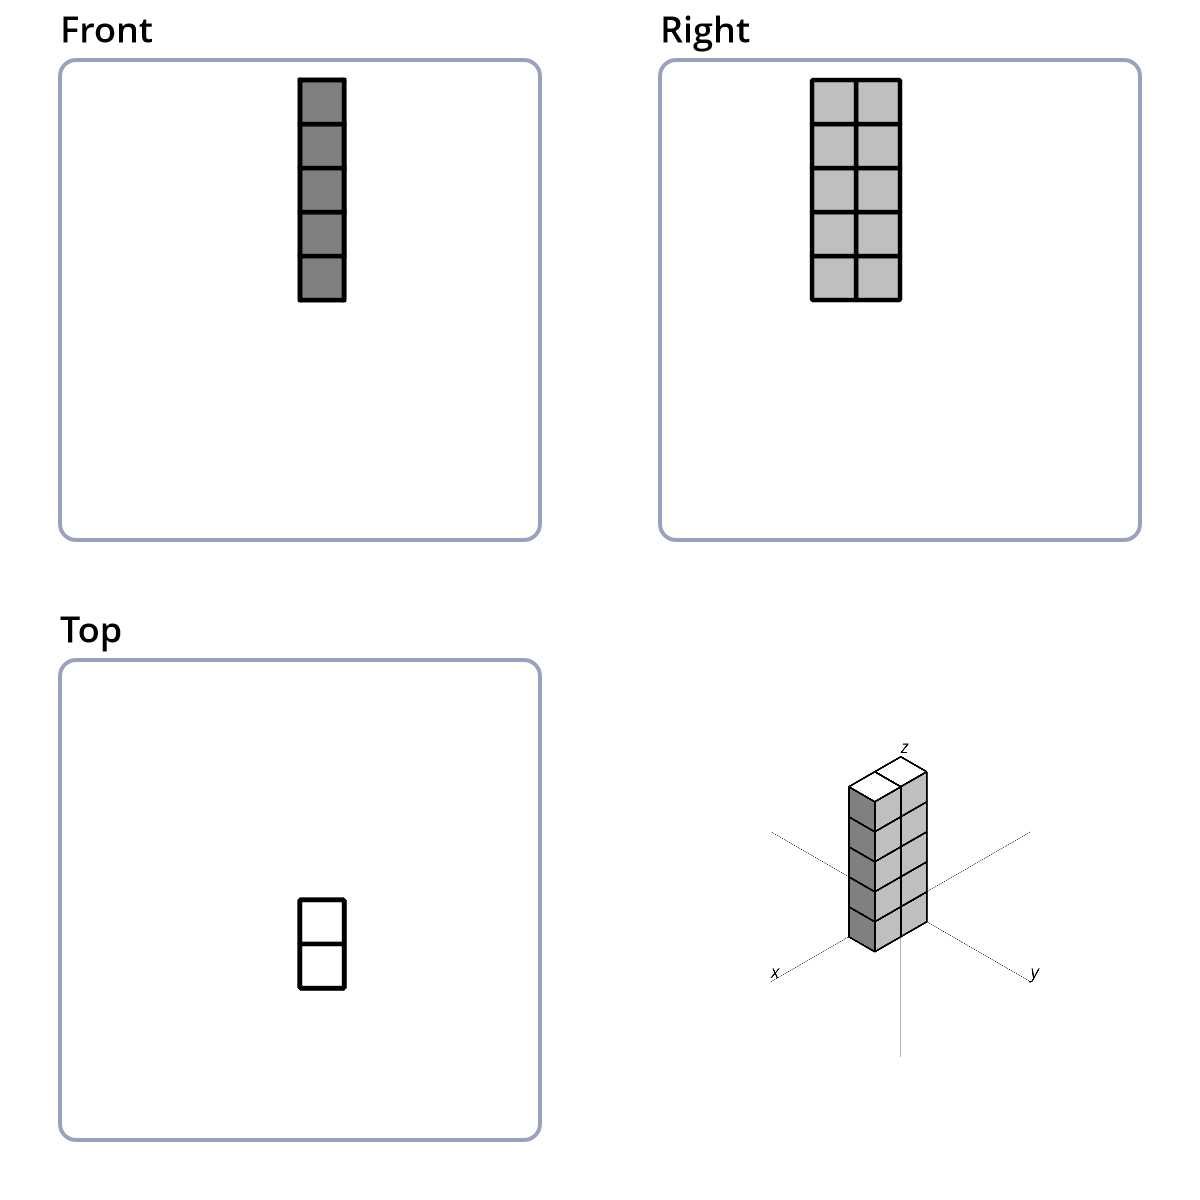
\includegraphics[scale=0.3]{iso_diagrams/o.png}
	\caption{Isometric of the O-pentomino.}
  \label{fig:iso-pent-o}
\end{figure}

\begin{figure}
	\centering
	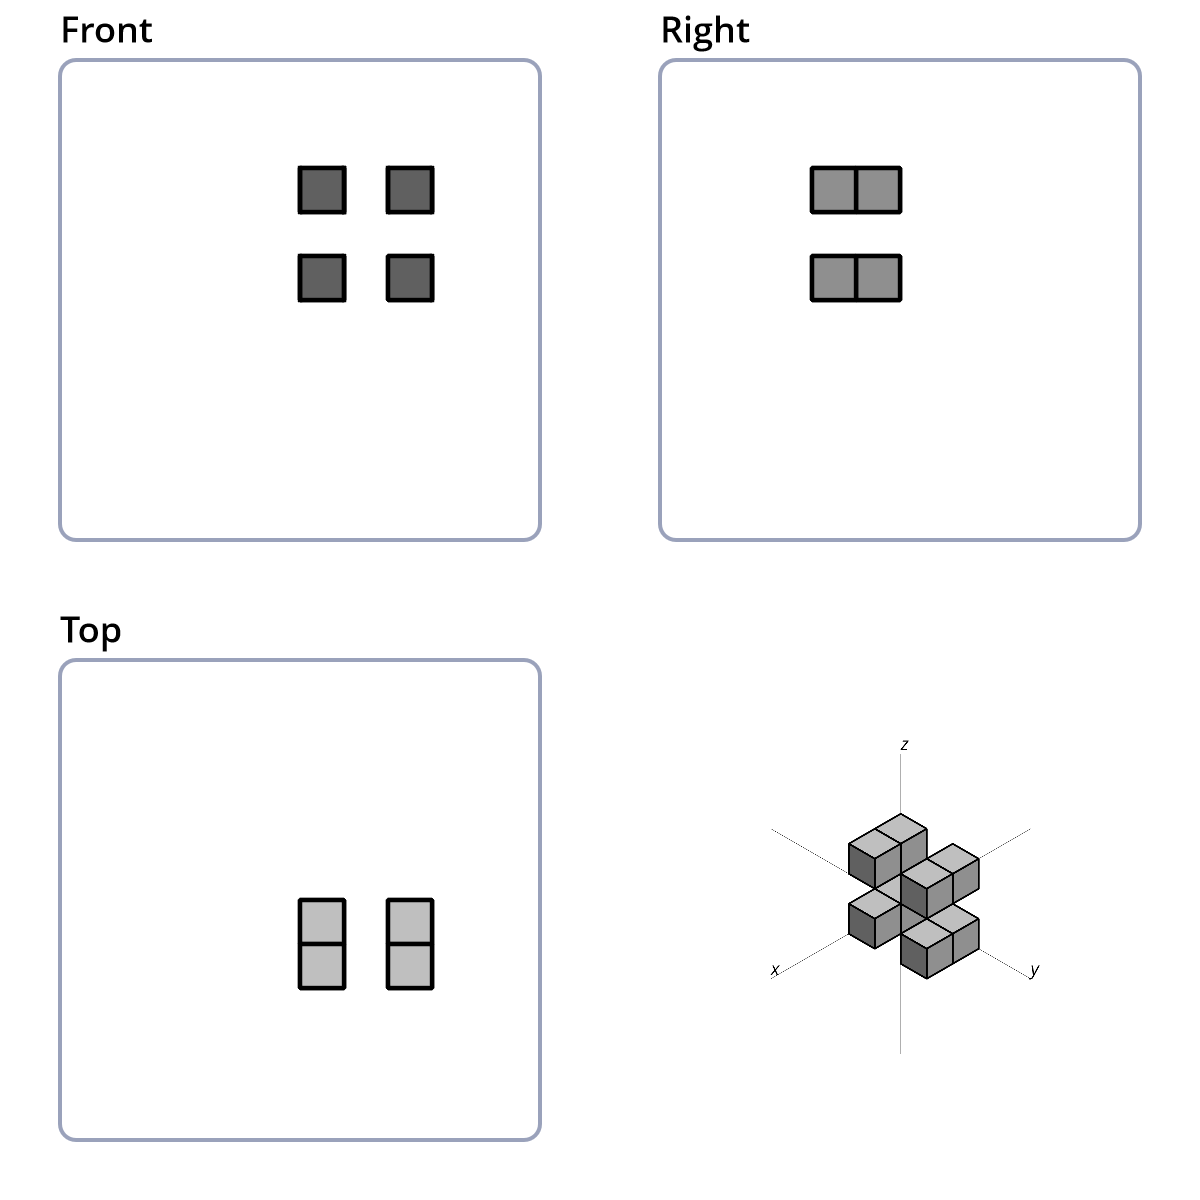
\includegraphics[scale=0.3]{iso_settings/osc_1.png}
	\caption{Isometric of oscillator-1.}
  \label{fig:iso-osc-1}
\end{figure}

\subsubsection{P-Pentomino}
This pentomino (see figure~\ref{fig:iso-pent-p}) is quite interesting; three
configurations can bee seen whithin less than 47 generations. The first one to
appear is a puffer train (see figure~\ref{fig:iso-puffer-1}), latter, the first
and most basic glider appears (see figure~\ref{fig:iso-glider-1}); finally,
another glider appears (see figure~\ref{fig:iso-glider-2}).

\begin{figure}
	\centering
	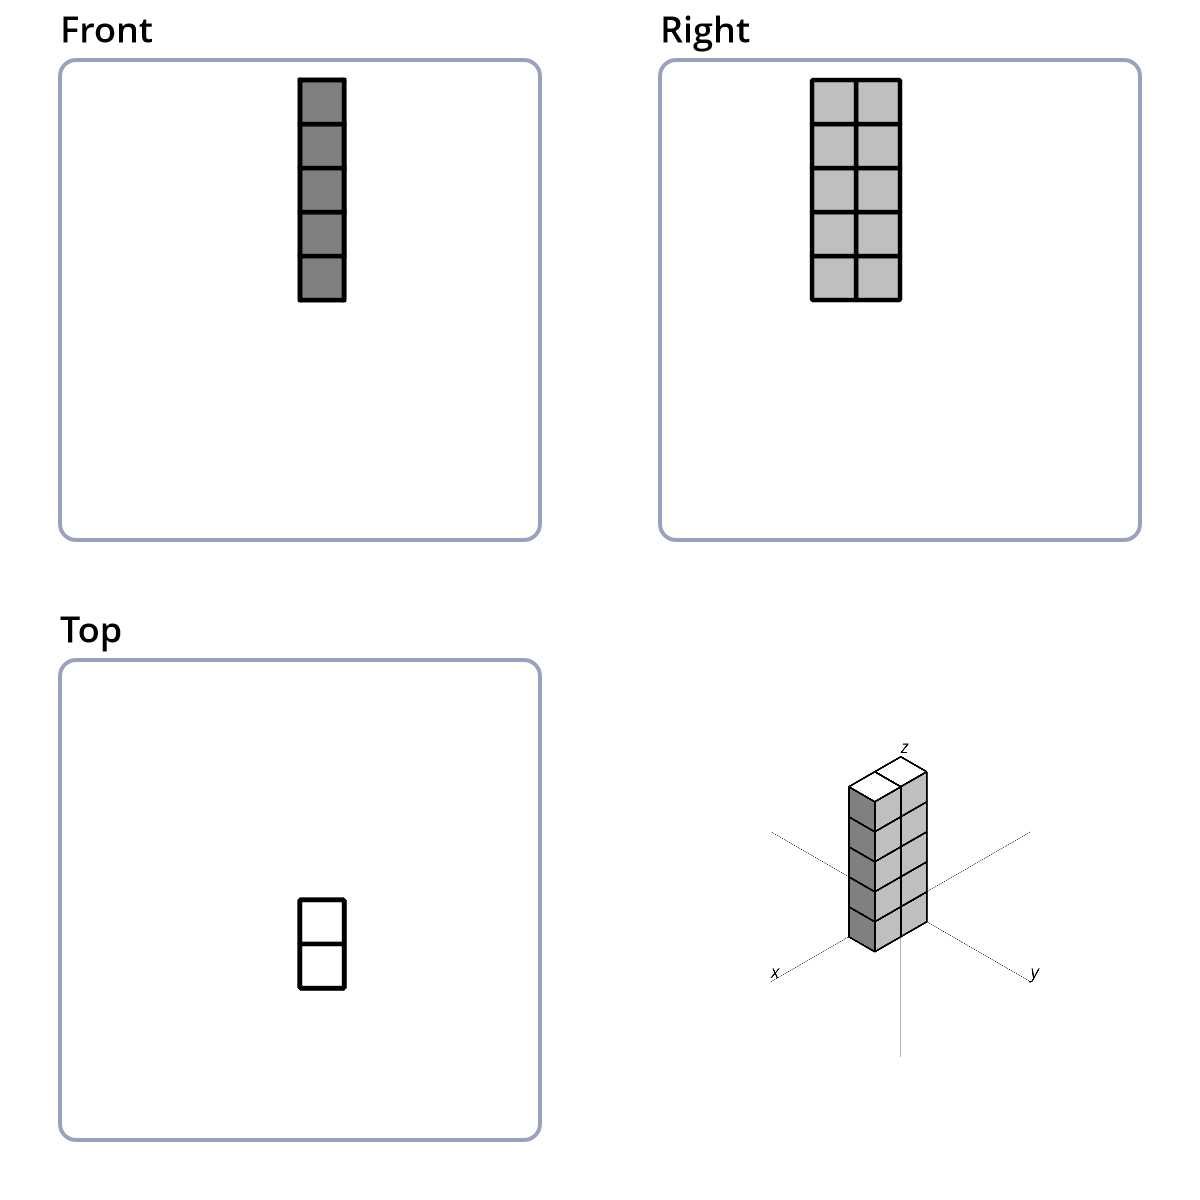
\includegraphics[scale=0.3]{iso_diagrams/o.png}
	\caption{Isometric of the P-pentomino.}
  \label{fig:iso-pent-p}
\end{figure}

\begin{figure}
	\centering
	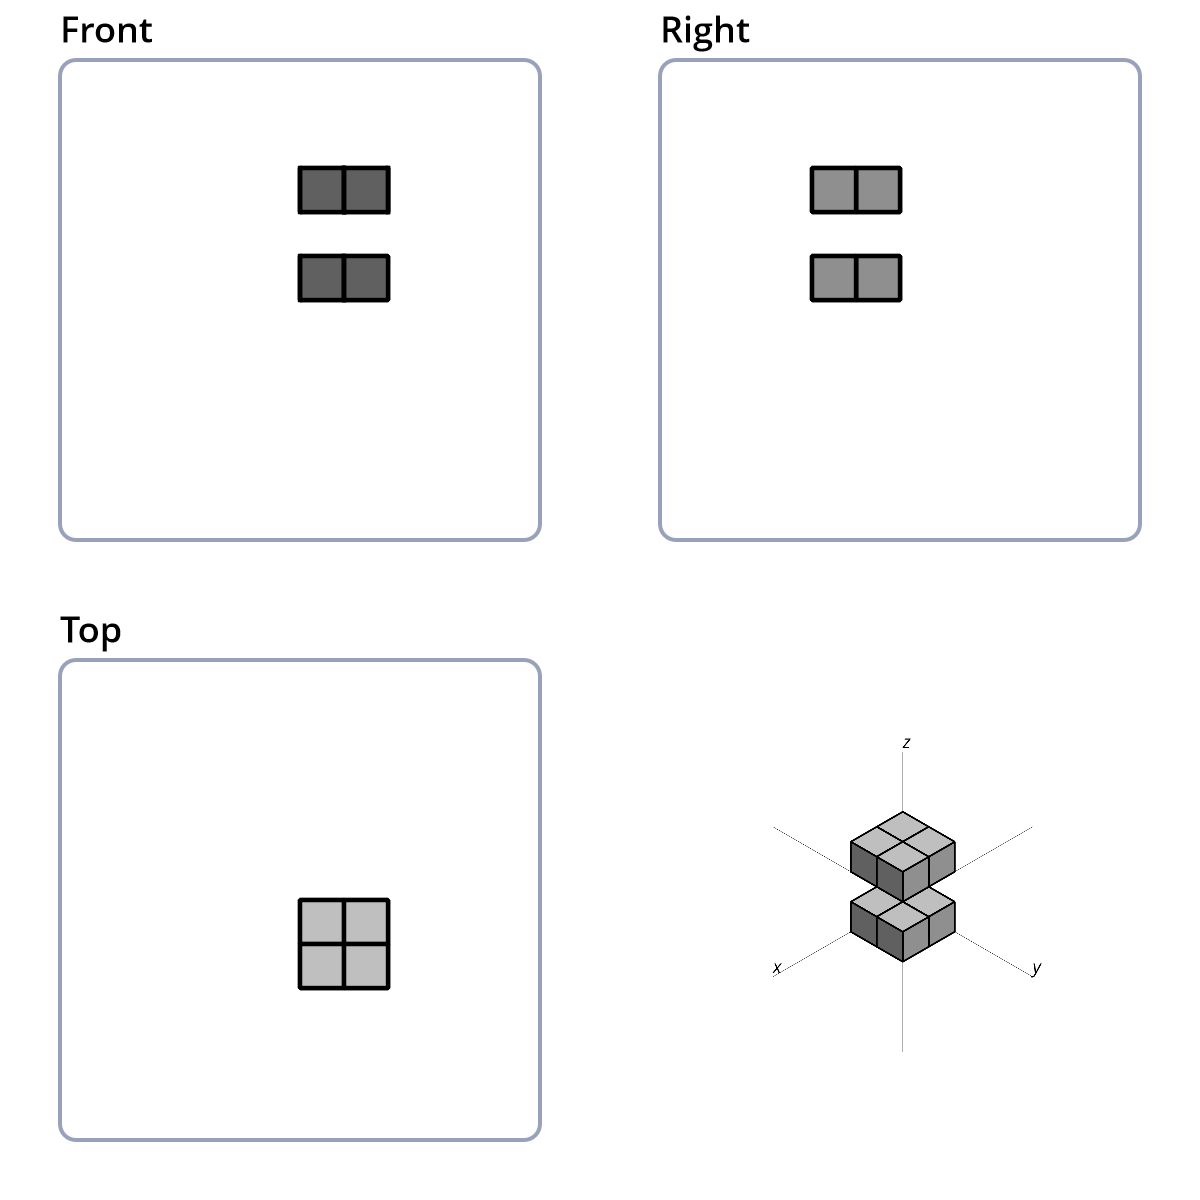
\includegraphics[scale=0.3]{iso_settings/puffer_1.png}
	\caption{Isometric of puffer-1.}
  \label{fig:iso-puffer-1}
\end{figure}

\begin{figure}
	\centering
	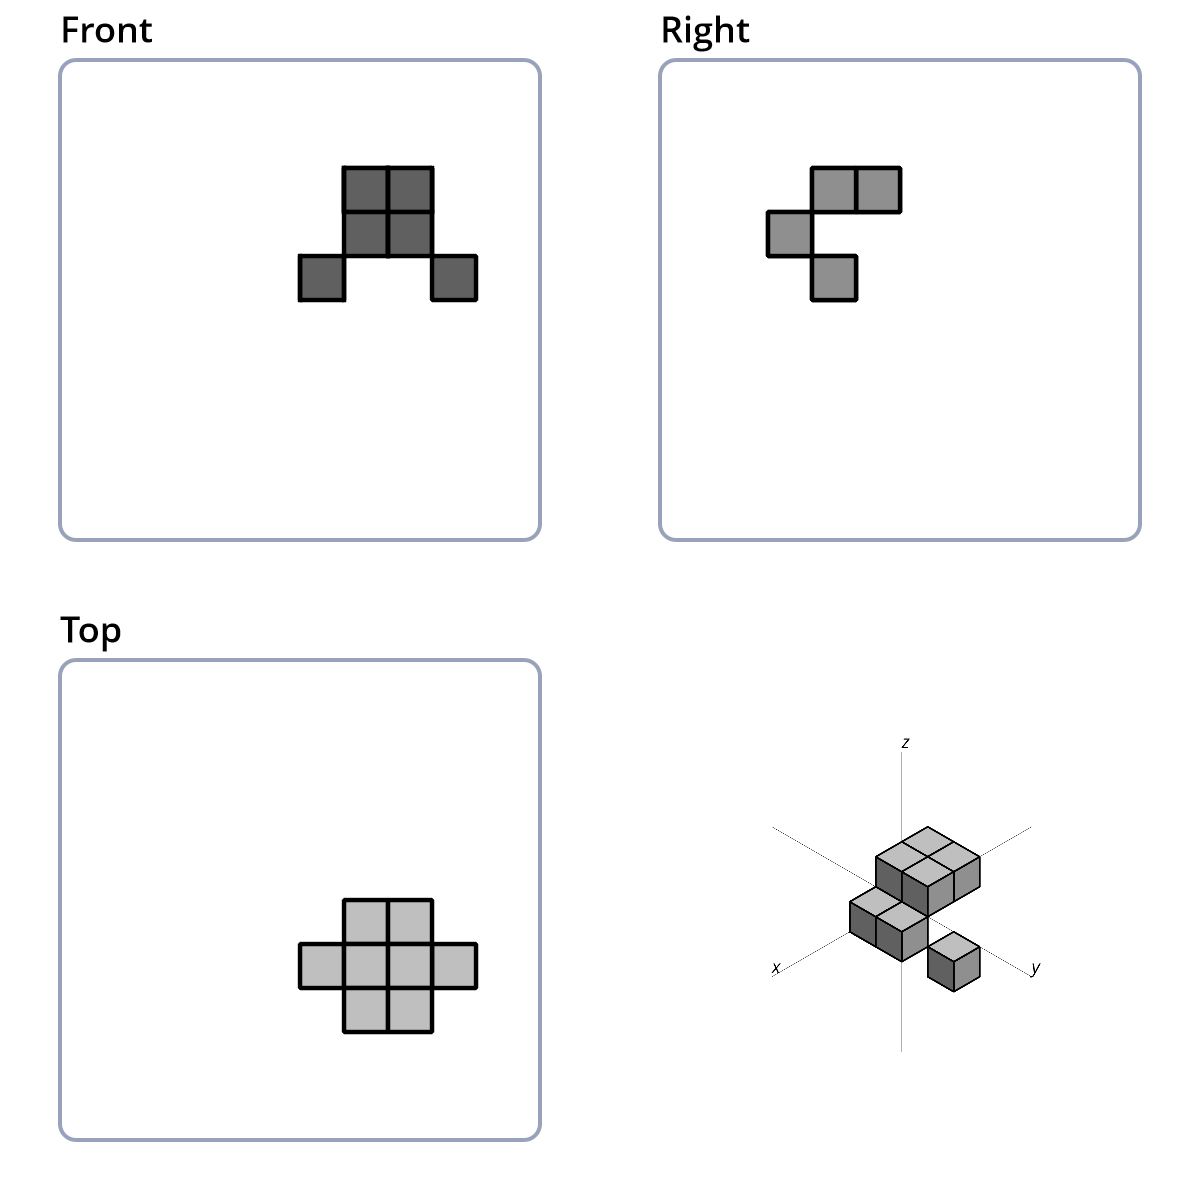
\includegraphics[scale=0.3]{iso_settings/glider_1.png}
	\caption{Isometric of glider-1.}
  \label{fig:iso-glider-1}
\end{figure}

\begin{figure}
	\centering
	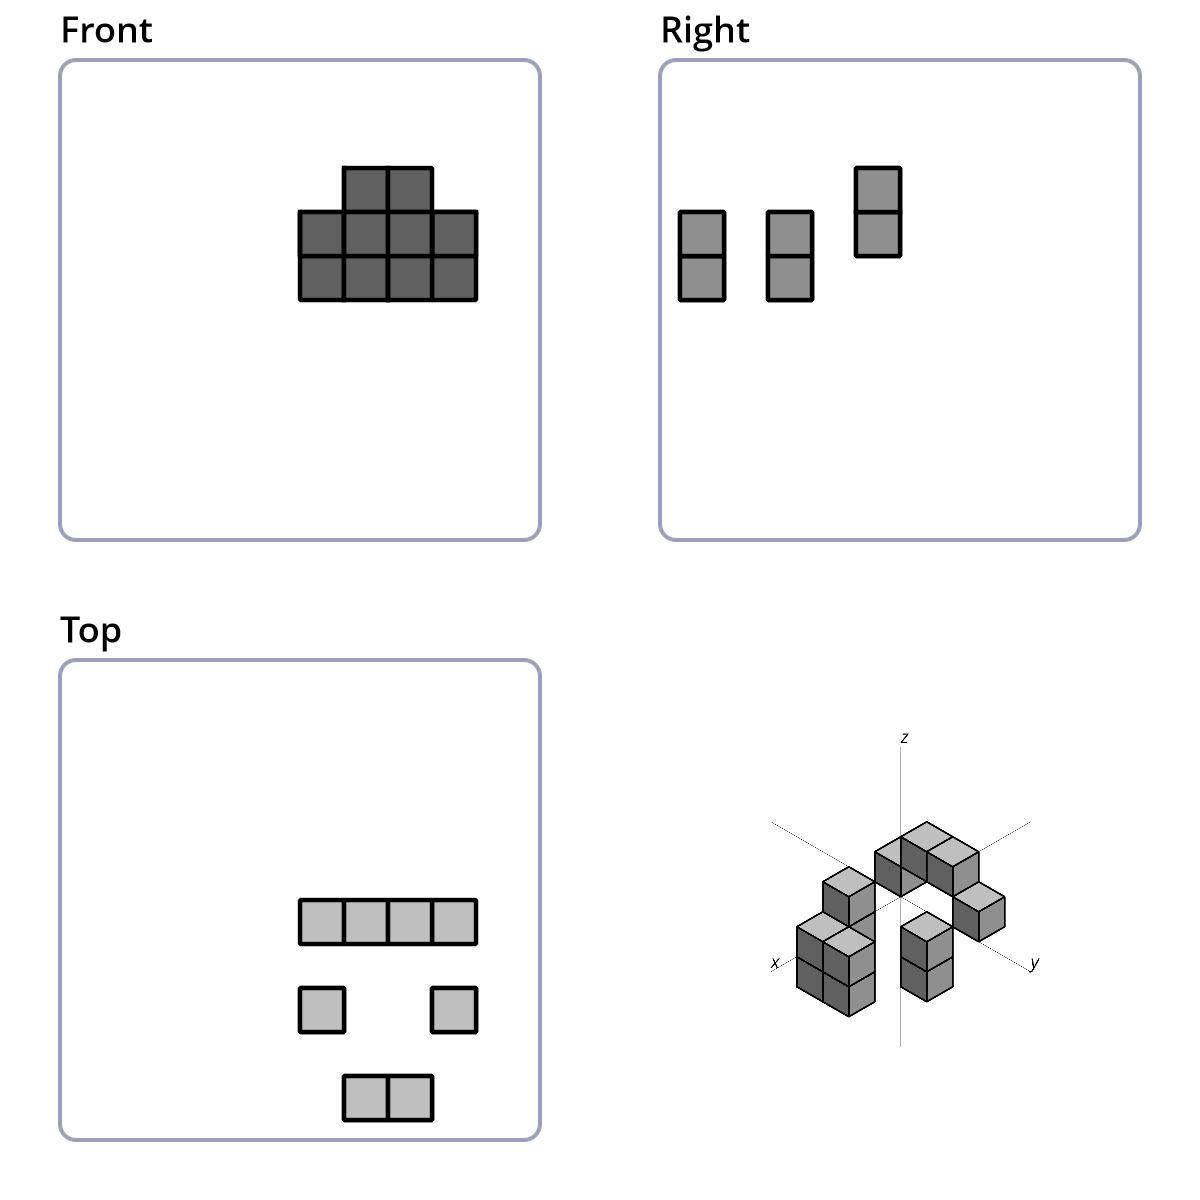
\includegraphics[scale=0.3]{iso_settings/glider_2.png}
	\caption{Isometric of glider-2.}
  \label{fig:iso-glider-2}
\end{figure}

\subsubsection{Q-Pentomino}
This pentomino (see figure~\ref{fig:iso-pent-q}),


\begin{figure}
	\centering
	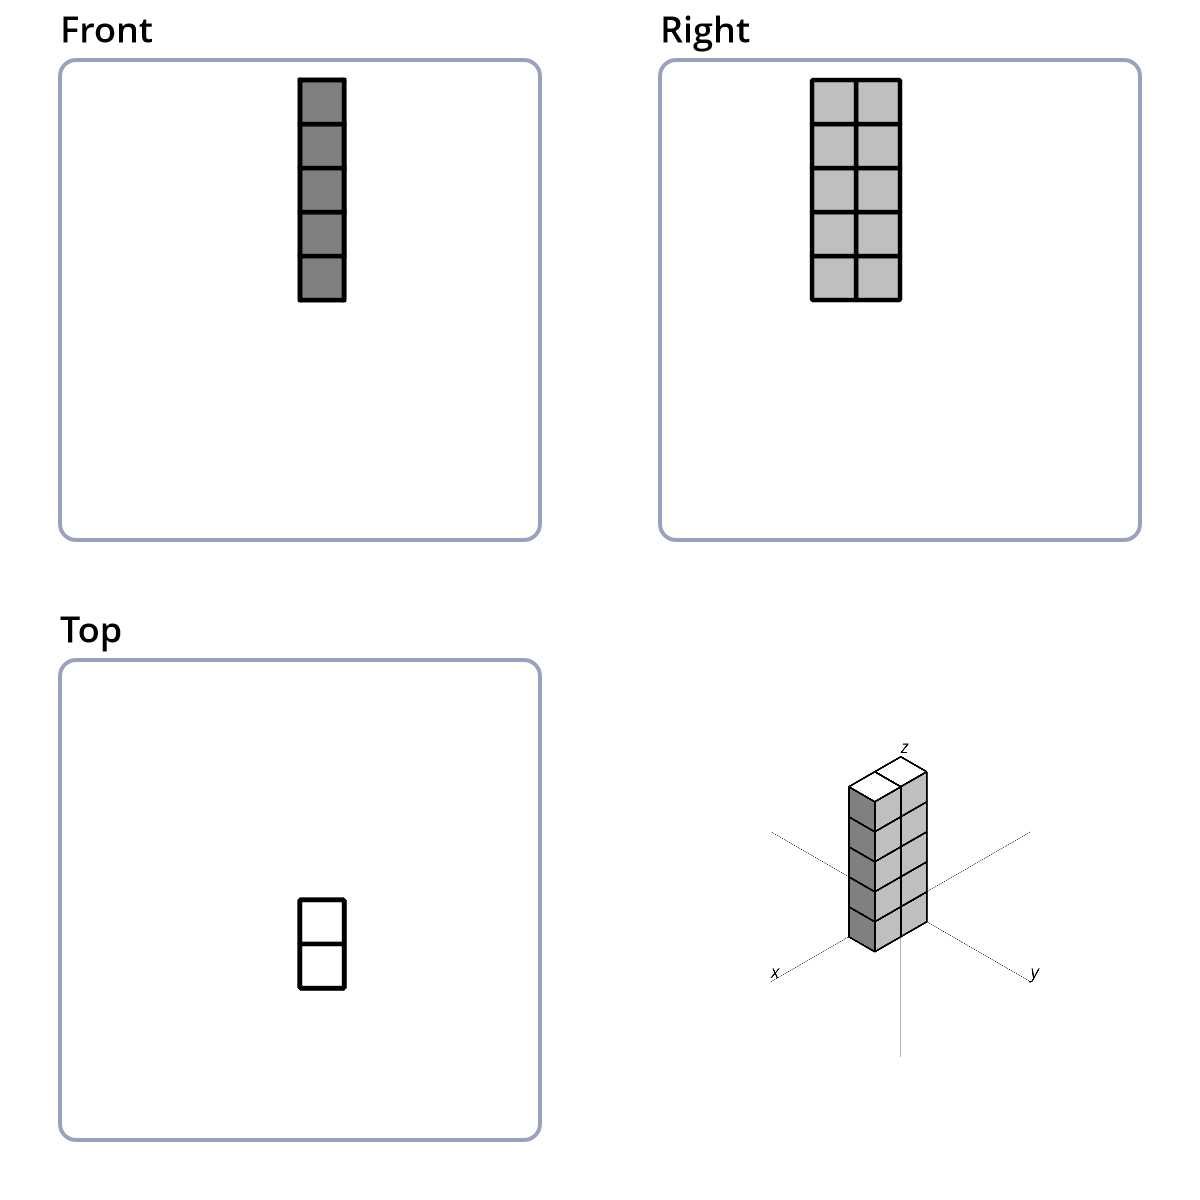
\includegraphics[scale=0.3]{iso_diagrams/o.png}
	\caption{Isometric of the Q-pentomino.}
  \label{fig:iso-pent-q}
\end{figure}
\subsubsection{R-Pentomino}
This pentomino (see figure~\ref{fig:iso-pent-r}),


\begin{figure}
	\centering
	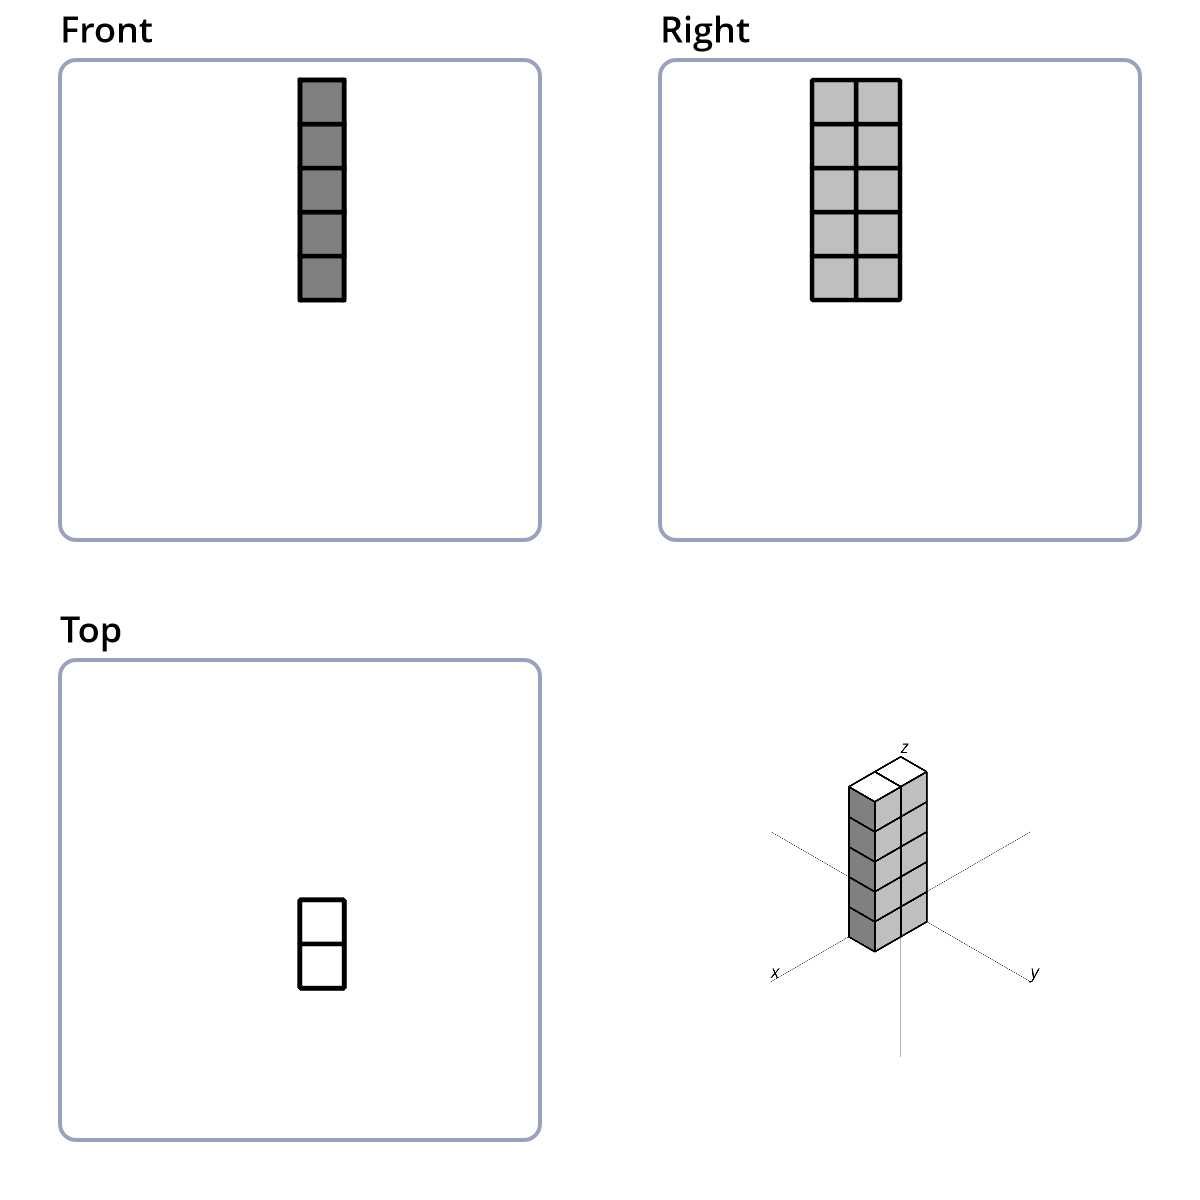
\includegraphics[scale=0.3]{iso_diagrams/o.png}
	\caption{Isometric of the R-pentomino.}
  \label{fig:iso-pent-r}
\end{figure}
\subsubsection{S-Pentomino}
This pentomino (see figure~\ref{fig:iso-pent-s}),


\begin{figure}
	\centering
	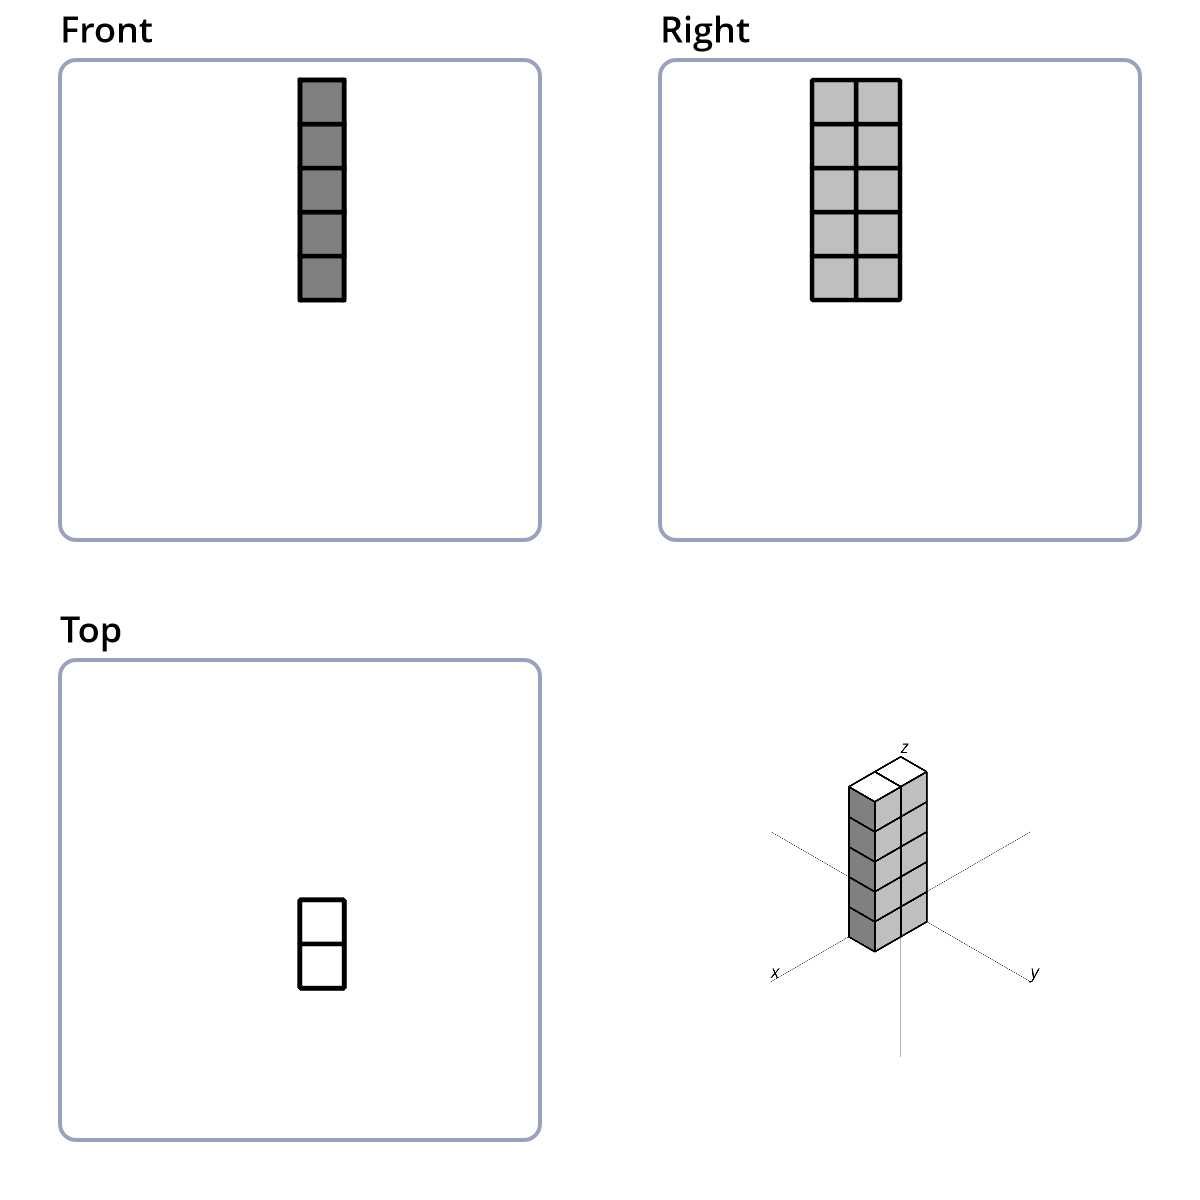
\includegraphics[scale=0.3]{iso_diagrams/o.png}
	\caption{Isometric of the S-pentomino.}
  \label{fig:iso-pent-s}
\end{figure}
\subsubsection{T-Pentomino}
This pentomino (see figure~\ref{fig:iso-pent-t}),


\begin{figure}
	\centering
	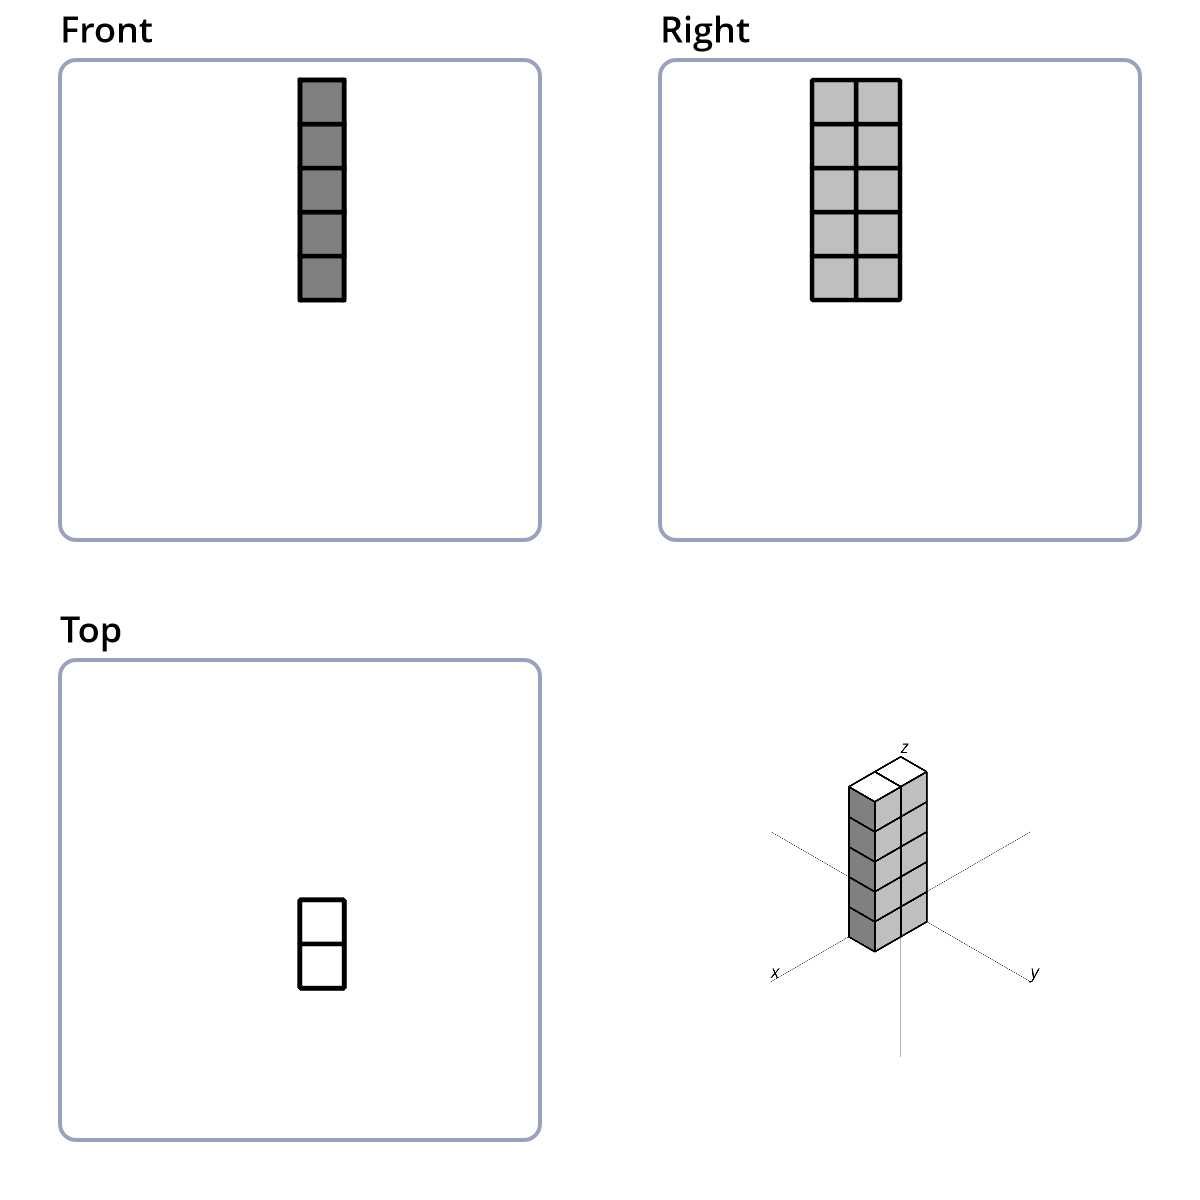
\includegraphics[scale=0.3]{iso_diagrams/o.png}
	\caption{Isometric of the T-pentomino.}
  \label{fig:iso-pent-t}
\end{figure}
\subsubsection{U-Pentomino}
This pentomino (see figure~\ref{fig:iso-pent-u}),


\begin{figure}
	\centering
	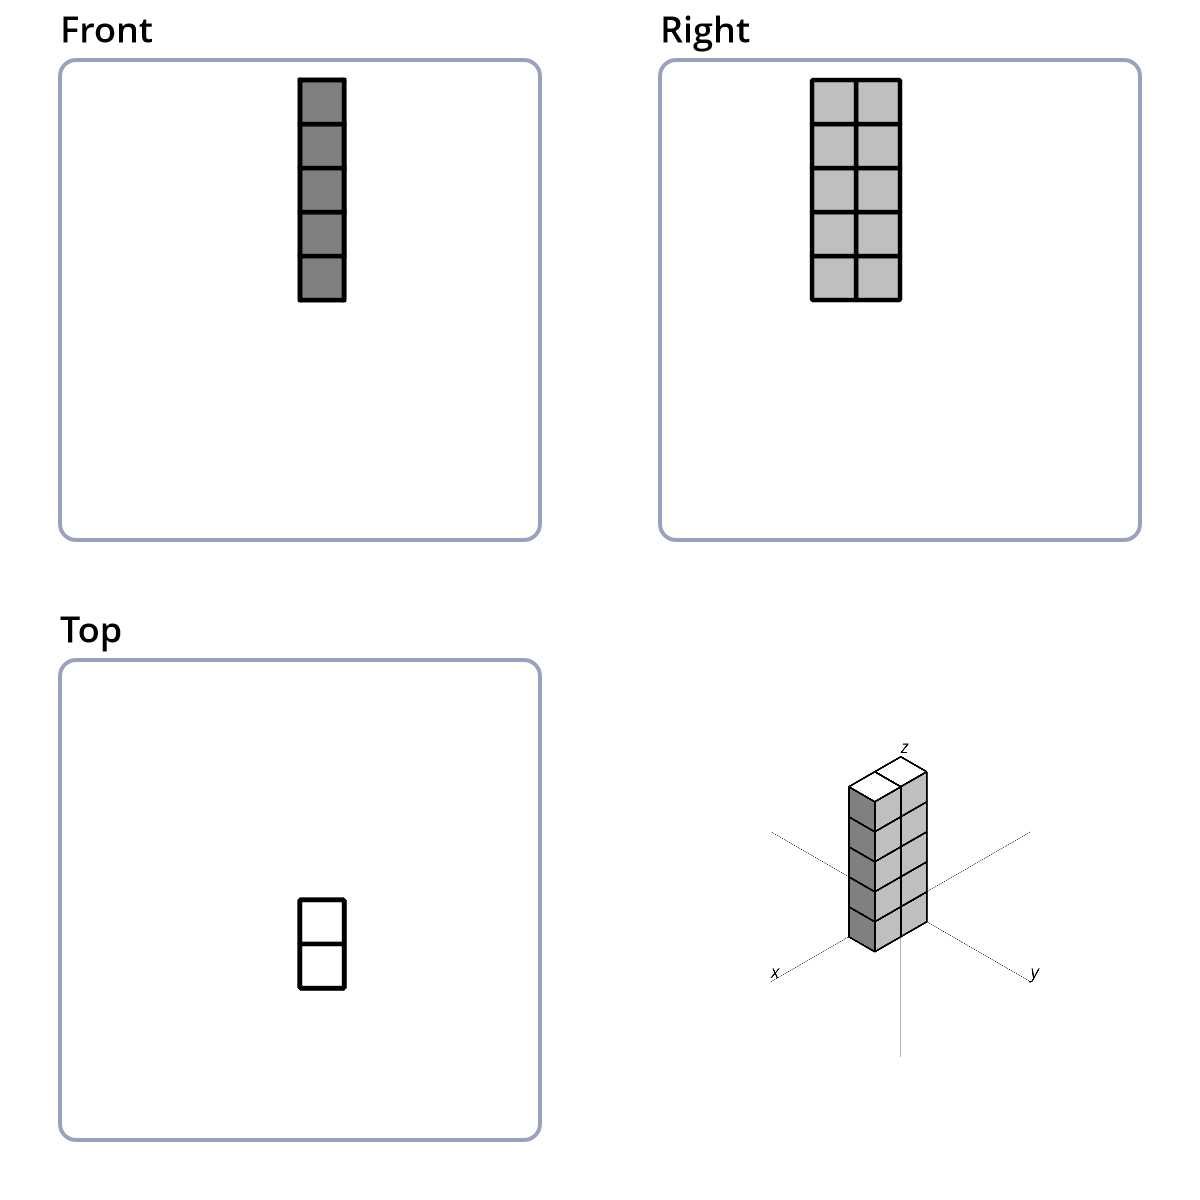
\includegraphics[scale=0.3]{iso_diagrams/o.png}
	\caption{Isometric of the U-pentomino.}
  \label{fig:iso-pent-u}
\end{figure}
\subsubsection{V-Pentomino}
This pentomino (see figure~\ref{fig:iso-pent-v}),


\begin{figure}
	\centering
	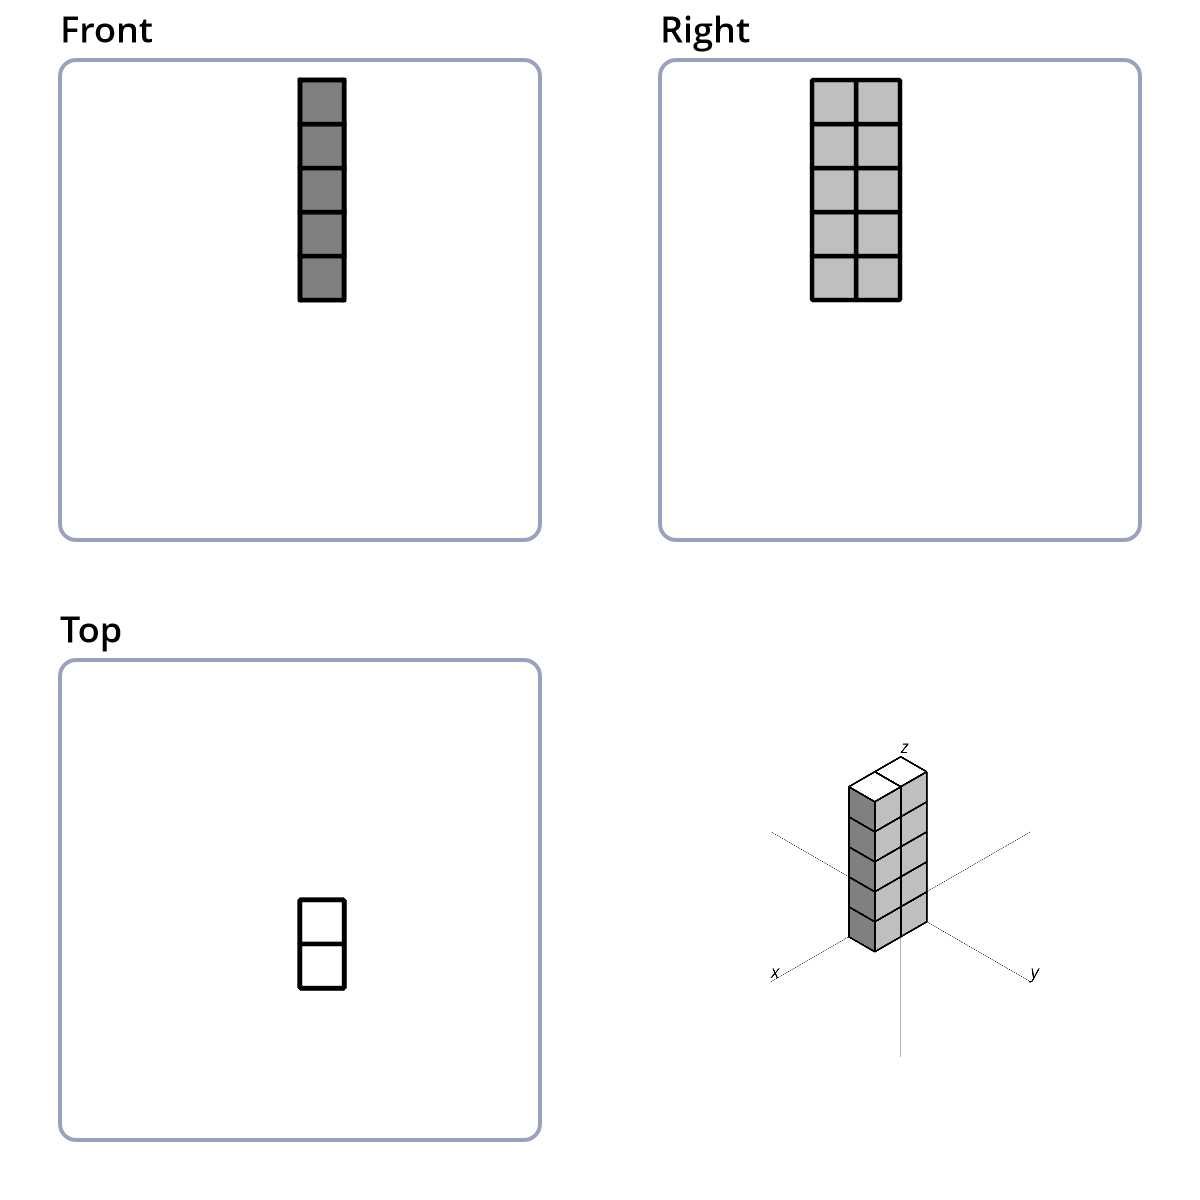
\includegraphics[scale=0.3]{iso_diagrams/o.png}
	\caption{Isometric of the V-pentomino.}
  \label{fig:iso-pent-v}
\end{figure}
\subsubsection{W-Pentomino}
This pentomino (see figure~\ref{fig:iso-pent-w}),


\begin{figure}
	\centering
	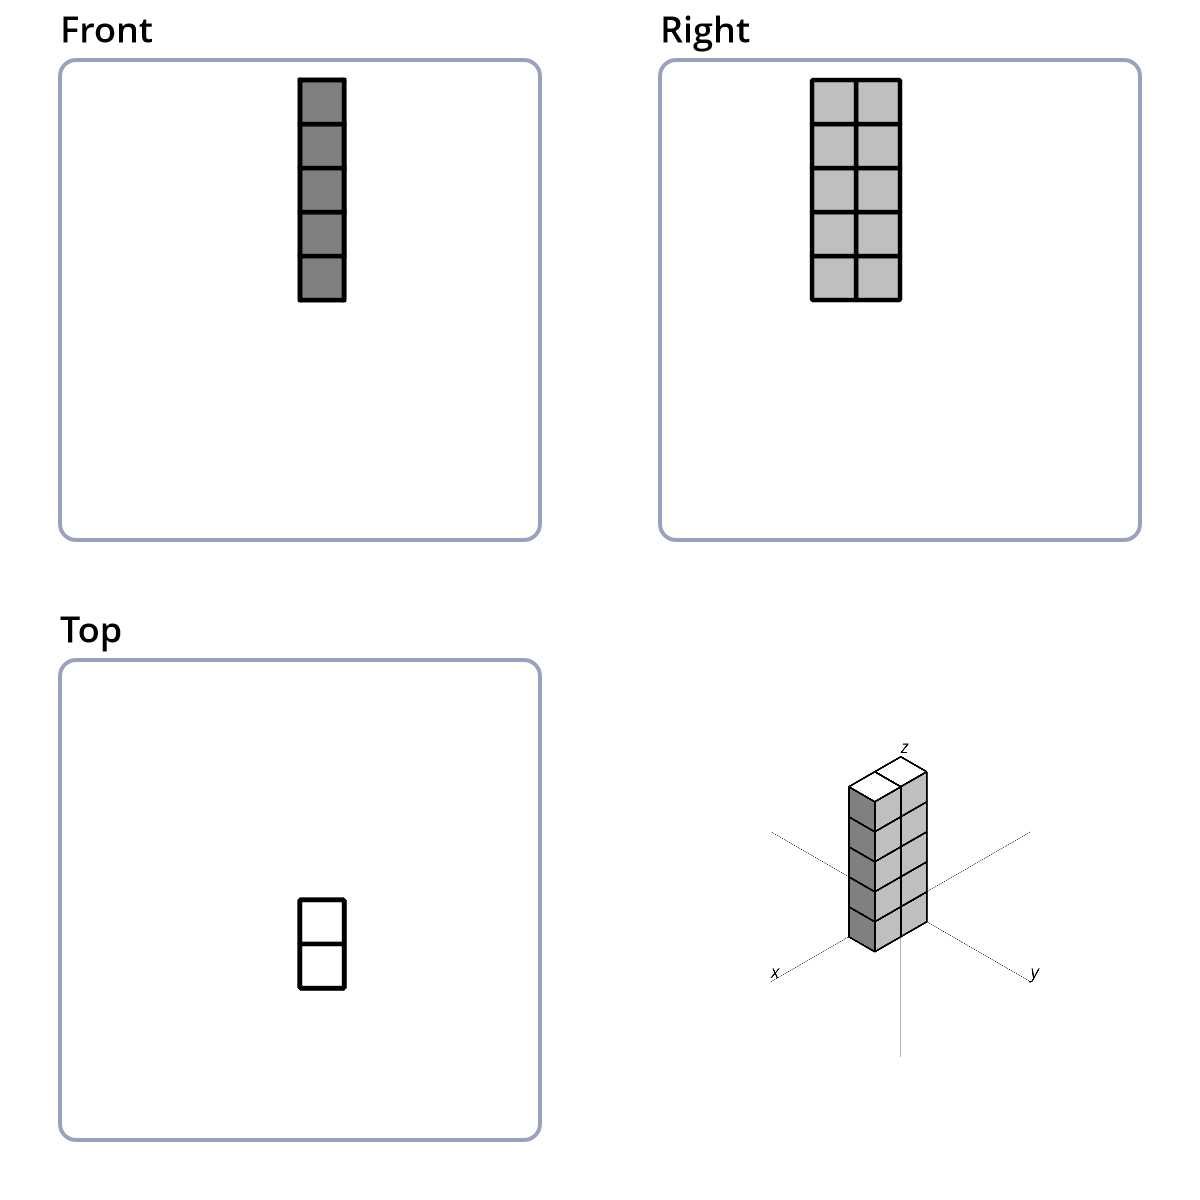
\includegraphics[scale=0.3]{iso_diagrams/o.png}
	\caption{Isometric of the W-pentomino.}
  \label{fig:iso-pent-w}
\end{figure}
\subsubsection{X-Pentomino}
This pentomino (see figure~\ref{fig:iso-pent-x}),


\begin{figure}
	\centering
	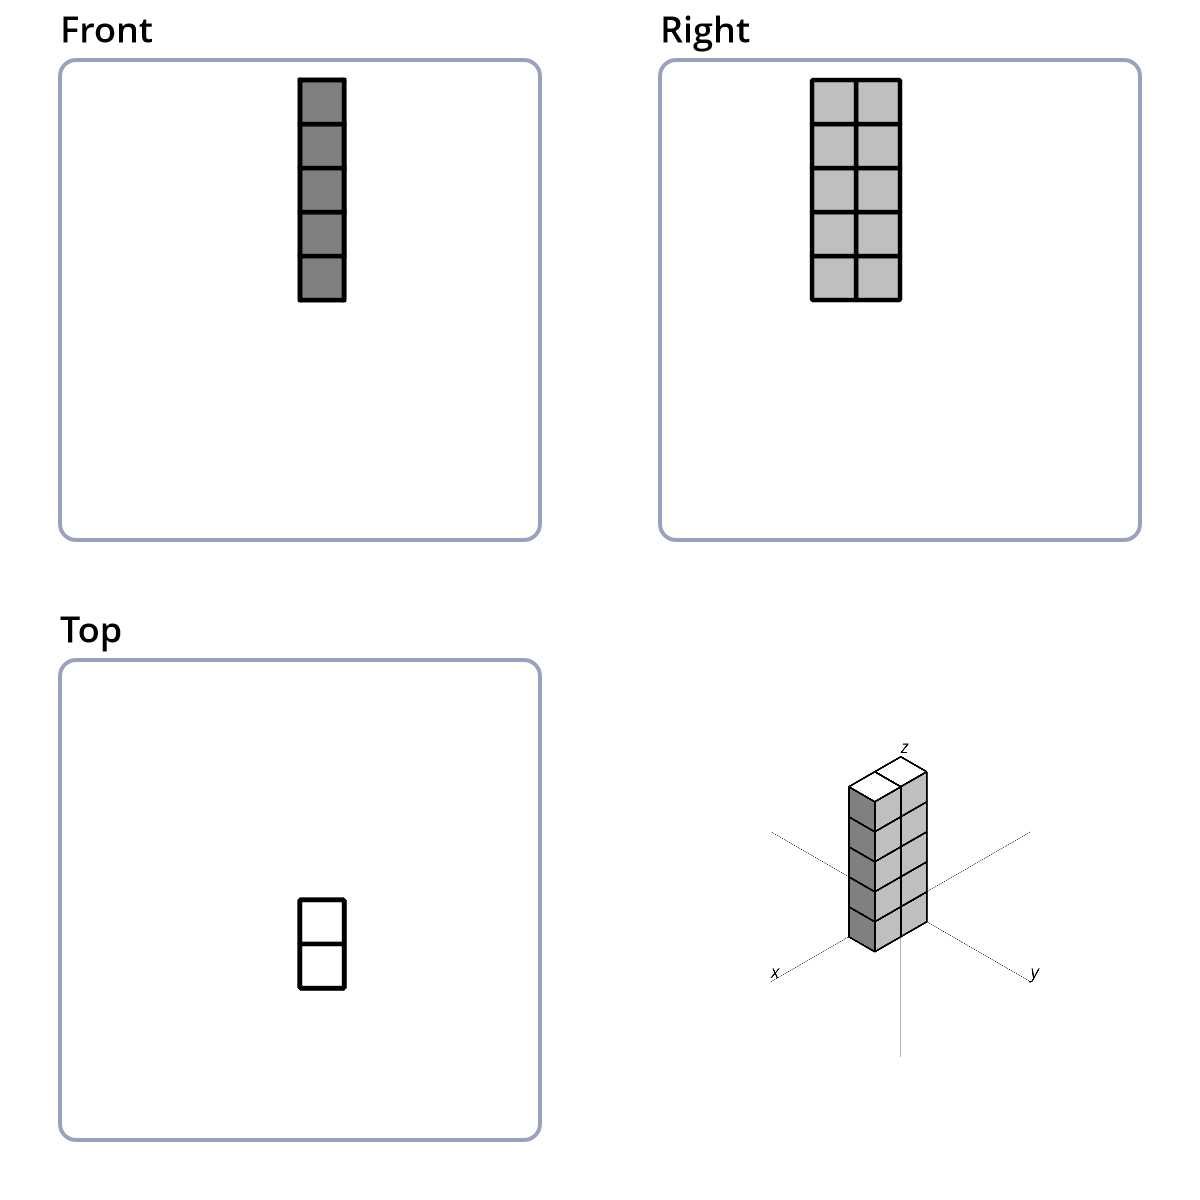
\includegraphics[scale=0.3]{iso_diagrams/o.png}
	\caption{Isometric of the X-pentomino.}
  \label{fig:iso-pent-x}
\end{figure}
\subsubsection{Y-Pentomino}
This pentomino (see figure~\ref{fig:iso-pent-y}),


\begin{figure}
	\centering
	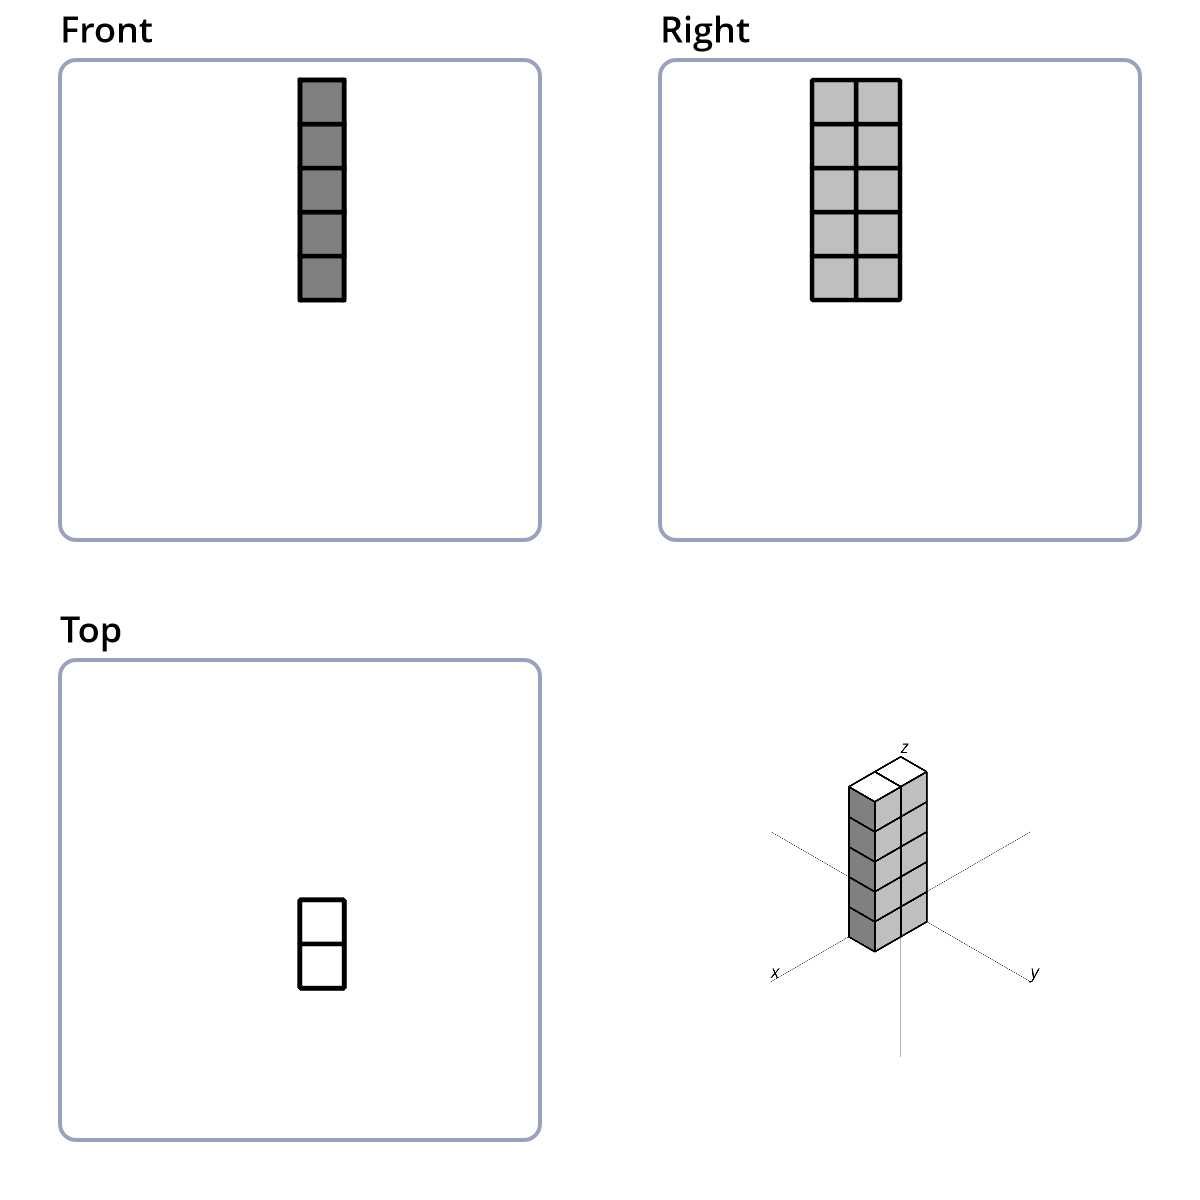
\includegraphics[scale=0.3]{iso_diagrams/o.png}
	\caption{Isometric of the Y-pentomino.}
  \label{fig:iso-pent-y}
\end{figure}
\subsubsection{Z-Pentomino}
This pentomino (see figure~\ref{fig:iso-pent-z}),


\begin{figure}
	\centering
	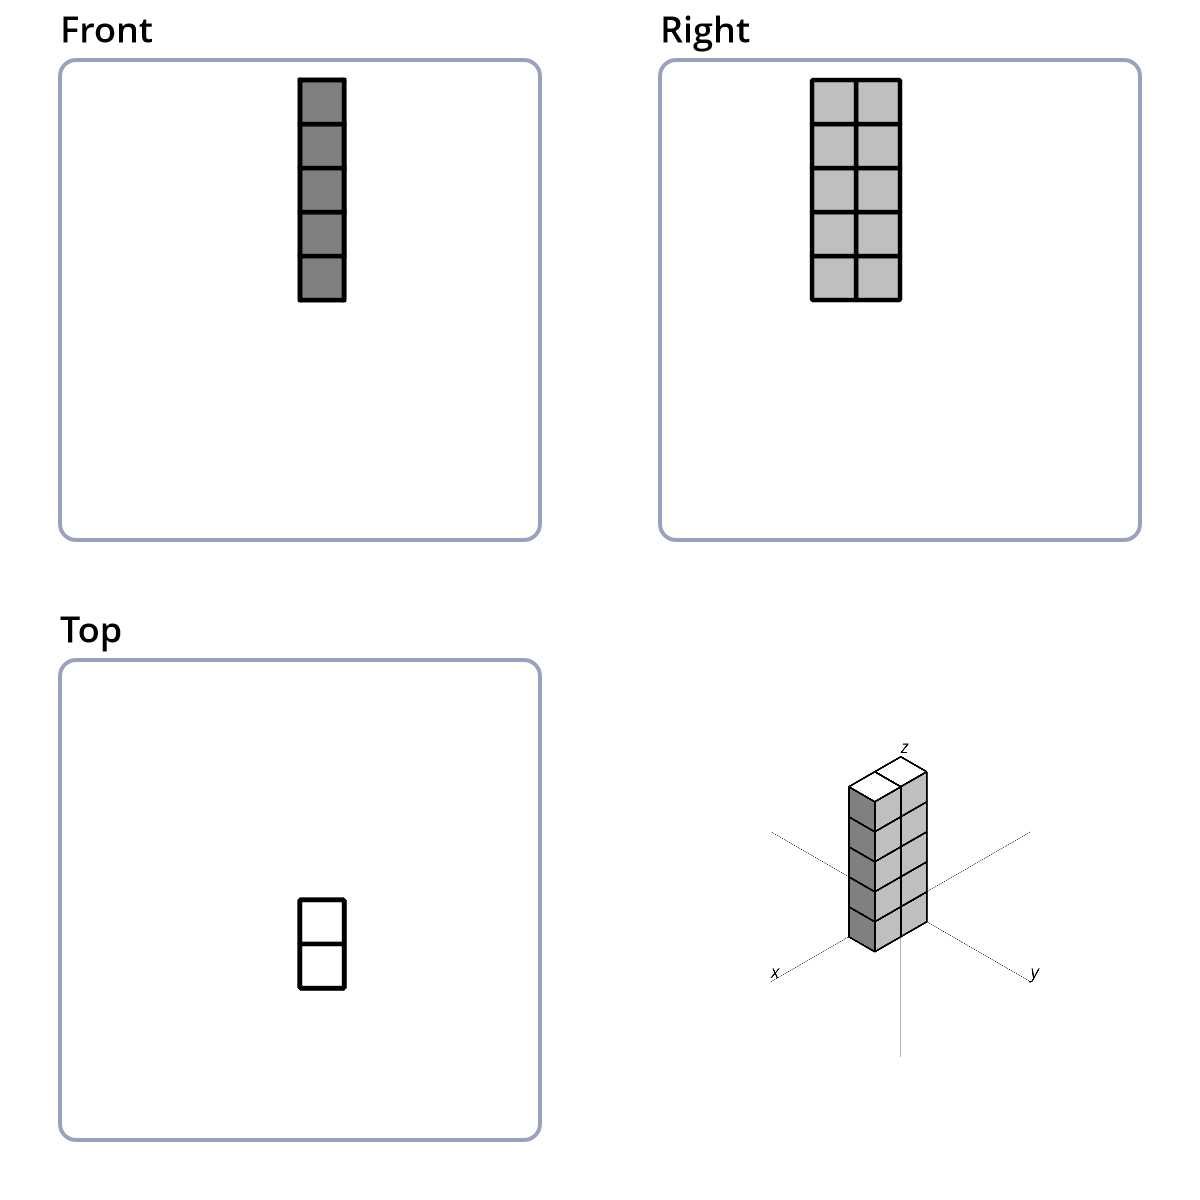
\includegraphics[scale=0.3]{iso_diagrams/o.png}
	\caption{Isometric of the Z-pentomino.}
  \label{fig:iso-pent-z}
\end{figure}
